%%%%%%%%%%%%%%%%%%%%%%%%%%%%%%%%%%%%%%%%%%%%%%%%%%%%%%
% Thanks to Xu Minghao's work                        %
% I modify it into uchicago version                  %
% to not make new bug, I don't alter "Ritsumeikan"   %
% keywords in file. Pls feel free to use             %
%%%%%%%%%%%%%%%%%%%%%%%%%%%%%%%%%%%%%%%%%%%%%%%%%%%%%%

%%%%%%%%%%%%%%%%%%%%%%%%%%%%%%%%%%%%%%%%%%%%%%%%%%%%%%
% A Beamer template for Ritsumeikan University       %
% Author: Ming-Hao Xu (Xu Minghao)                   %
% Date:   April 2022.                                %
% LPPL Licensed.                                     %
%%%%%%%%%%%%%%%%%%%%%%%%%%%%%%%%%%%%%%%%%%%%%%%%%%%%%%

\documentclass[10pt]{beamer}
\usepackage[T1]{fontenc}

\usetheme[progressbar=frametitle]{metropolis}
%\usetheme{Warsaw}
\metroset{block=fill}

\usepackage{lipsum}  
\usepackage{natbib}
\usepackage{ragged2e}  
\usepackage{listings}
\usepackage[utf8]{inputenc}
\usepackage{array}
\usepackage{amsmath}
\usepackage{multirow}
\usepackage{subcaption}
\usepackage[svgnames]{xcolor}
\usepackage{gensymb}
\setbeamertemplate{caption}[numbered]

\setcitestyle{round} % for rounded brackets

% \renewcommand{\figurename}{Fig.}

\hypersetup{
    colorlinks = true,
    linkcolor=,
    urlcolor = blue,
    citecolor=black
}

\definecolor{codegreen}{rgb}{0,0.6,0}
\definecolor{codegray}{rgb}{0.5,0.5,0.5}
\definecolor{codepurple}{rgb}{0.58,0,0.82}
\definecolor{backcolour}{rgb}{0.95,0.95,0.92}

\lstdefinestyle{mytex}{
    language=tex,
    backgroundcolor=\color{backcolour},   
    commentstyle=\color{codegreen},
    keywordstyle=\color{blue},
    numberstyle=\tiny\color{codegray},
    stringstyle=\color{codepurple},
    basicstyle=\ttfamily\scriptsize,
    breakatwhitespace=false,         
    breaklines=true,                 
    captionpos=b,                    
    keepspaces=true,                 
    % numbers=left,                    
    % numbersep=5pt,                  
    showspaces=false,                
    showstringspaces=false,
    showtabs=false,                  
    tabsize=2,
    morekeywords={begin, maketitle, title, author, title, usepackage, documentclass, date, today, chapter, section, subsection, label, lipsum, Large, normalsize, raggedleft, justifying, fancyhead, fancyfoot, renewcommand, chaptermark, markboth, MakeUppercase, thesection, thechapter, chaptername, sectionmark, pagestyle, markright, includegraphics, caption, vspace, linewidth, doublespacing, linenumbers, makeatletter, theequation, renewcommand, arabic, makeatother, clearpage, includepdf, geometry, bibliography, bibliographystyle, subsubsection, addcontentsline, addstarredchapter, tableofcontents, setcounter, minitoc, dominitoc, url, href, footnote}
}

\lstdefinestyle{bash}{
    language=bash,
    backgroundcolor=\color{backcolour},   
    commentstyle=\color{codegreen},
    % keywordstyle=\color{magenta},
    % numberstyle=\tiny\color{codegray},
    % stringstyle=\color{codepurple},
    basicstyle=\ttfamily\footnotesize,
    breakatwhitespace=false,         
    breaklines=true,                 
    captionpos=b,                    
    keepspaces=true,                 
    % numbers=left,                    
    % numbersep=5pt,                  
    showspaces=false,                
    showstringspaces=false,
    showtabs=false,                  
    tabsize=2}


\author{Nicolas Barrier}
\title{Introduction to \LaTeX}
% \subtitle{CCNU Beamer Theme}
\institute{
    UMR MARBEC
}
\date{\today}

\definecolor{deepblue}{rgb}{0,0,0.5}
\definecolor{ccnuMainColor}{RGB}{0,86,109}
\definecolor{deepgreen}{rgb}{0,0.5,0}
\definecolor{halfgray}{gray}{0.55}

\begin{document}
\lstset{style=mytex}

\frame{\titlepage}

% comportement special en debut de section
\AtBeginSection[]
{
  \begin{frame}<beamer>
    % afficher le sommaire
    \frametitle{Table of content}
    % section (courante en surbrillance), pas de sous-section
    \tableofcontents[current,hideallsubsections]
  \end{frame}
}

% comportement special en debut de sous-section
% \AtBeginSubsection[]
% {
%   \begin{frame}<beamer>
%     \frametitle{Table of content}
%     % section courante
%     % sous-sections de la section courante
%     \tableofcontents[sectionstyle=show/shaded,subsectionstyle=show/shaded/hide]
%   \end{frame}
% }


\section{Introduction}
\subsection{Description}

\begin{frame}{What is \LaTeX{}?}

\emph{\LaTeX{} is a software system for typesetting documents.} (Source: \href{https://en.wikipedia.org/wiki/LaTeX}{Wikipedia}). In short: you write code, you obtain nicely formatted documents (reports, articles, presentations) \\

\begin{block}{Pros}
\begin{itemize}
\item{Free and cross-platform (Windows, Unix, Mac Os)}
\item{Really nice rendering}
\item{Typesetting of mathematical equations}
\item{Can split a large document into different parts}
\item{Large community and a lot of \LaTeX{} compatible tools}
\item{Easy management of bibiography}
\end{itemize}
\end{block}

\begin{alertblock}{Cons}
\begin{itemize}
\item{You need to learn the syntax}
\item{Layout modifications is difficult for beginners}
\end{itemize}

\end{alertblock}

\end{frame}

\begin{frame}[fragile]{Install \LaTeX{}}
For Windows: download and install the \href{https://mirror.ctan.org/systems/texlive/tlnet/install-tl-windows.exe}{install-tl-windows.exe} program\\
\vspace{1em}

For Mac Os X: download and install the \href{https://mirror.ctan.org/systems/mac/mactex/MacTeX.pkg}{MacTex.pkg} file.\\
\vspace{1em}

For Unix/Linux: open a terminal and type:
\begin{lstlisting}[style=bash]
sudo apt install texlive-base
\end{lstlisting}

\end{frame}

\begin{frame}[fragile]{Some \LaTeX{} editors}

\LaTeX{} source files are text files with a \verb+.tex+ extension, which can be edited with any text editors. However, some editors are specifically made for \LaTeX{}:\\

\begin{itemize}
 \item{\href{https://www.overleaf.com/}{Overleaf}: online editor, collaborative writing, automatic compile, it also provides a nice \href{https://www.overleaf.com/learn/latex}{documentation} and numerous \href{https://www.overleaf.com/latex/templates}{templates} (thesis, articles, presentations)}
 \item{\href{https://www.xm1math.net/texmaker/}{Texmaker}: free and open-source cross-platform editor}
 \item{\href{https://texstudio.sourceforge.net/}{Texstudio}: free and open-source cross-platform editor, forked from Texmaker}
 
\end{itemize}

For a complete list, see \href{https://en.wikipedia.org/wiki/Comparison_of_TeX_editors}{here}...

\end{frame}

\subsection{Getting started}

\begin{frame}[fragile]{Document structure}

A \LaTeX{} file is separated into two parts:
\begin{itemize}
    \item A header: it contains the document definition (article, book, presentation), the packages used, the author name, the date, the title, etc. It basically controls the final rendering of the document.
    \item The content of the document, which is contained between a \verb+\begin{document}+ and a \verb+\end{document}+ statement.
\end{itemize}

The code is made of \emph{blocks}, which are always contained between a \verb+begin+ and \verb+end+ statements. The main block is the \verb+document+ block.

\end{frame}

\begin{frame}[fragile]{Document structure: example}
For a simple document:

\begin{lstlisting} 
%%%%%%%%  header 
% document definition
\documentclass[10pt]{book}

% inclusion of the package 
\usepackage[utf8]{inputenc}

% defining some informations
\author{Nicolas Barrier}
\title{My first document}
\date{\today}

%%%%%%%% document
\begin{document}
\maketitle  % command to write the title page
\end{document}
\end{lstlisting}

Optional arguments are provided between \verb+[ ]+, compulsory arguments are provided between \verb+{ }+

\end{frame}

\begin{frame}[fragile]{Document compilation}

To generate the PDF document from the Terminal, type:
\begin{lstlisting}[style=bash]
pdflatex tex_example.tex
\end{lstlisting}

To generate the PDF document from Texmaker (Fig. \ref{fig-texmaker-compile}):
\begin{itemize}
    \item Click on the \verb+PDFLaTeX+ arrow \textcolor{red}{(1)}
    \item Click on the \verb+View PDF+ arrow \textcolor{blue}{(2)}
\end{itemize}

\begin{figure}
    \centering
    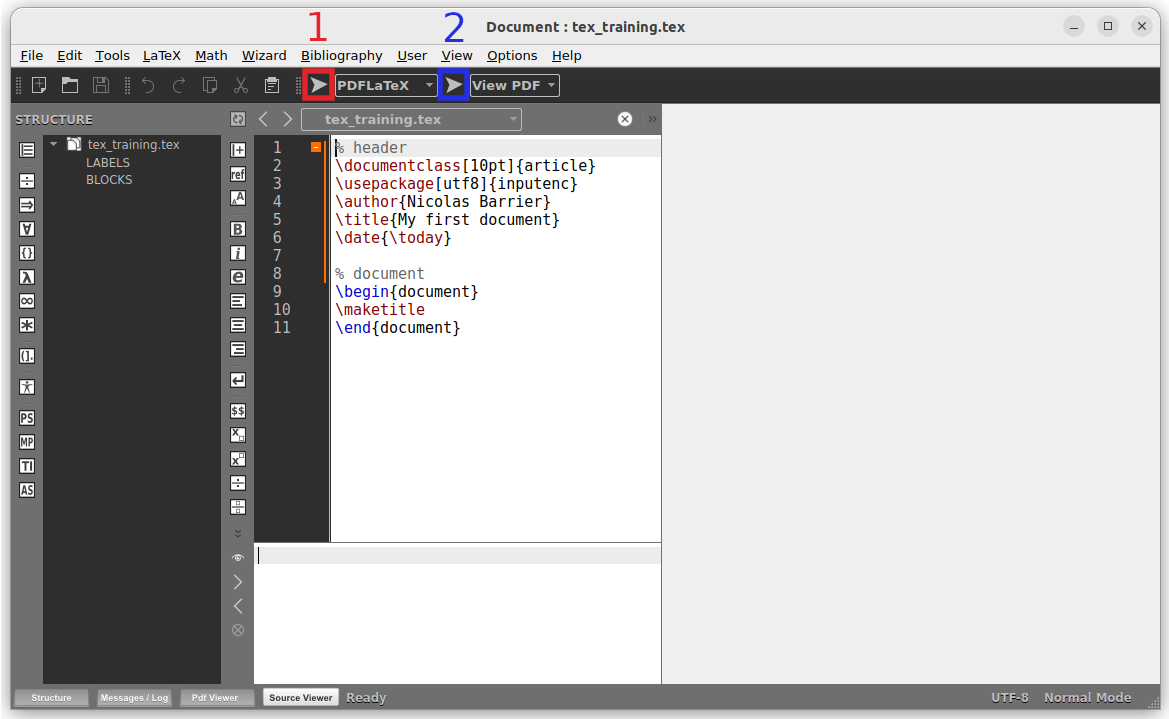
\includegraphics[width=0.5\linewidth]{figs/texmaker-1.png}
    \caption{Compilation using Texmaker}
    \label{fig-texmaker-compile}
\end{figure}

\end{frame}

\begin{frame}[fragile]{Usefull packages}

External packages can be included using the \lstinline{\usepackage} command. 
Some useful packages are listed below:

\footnotesize

\begin{table}
\begin{tabular}{m{5em}m{25em}}
    \verb+hyperref+ & inclusion of external links\\
    \verb+natbib+ & bibliography\\
    \verb+ragged2e+ & for text alignment\\
    \verb+listings+ & code inclusion (R, Python, etc.)\\
    \verb+babel+ & for french documents\\
    \verb+xcolor+ & colors\\
    \verb+graphicx+& figures \\
    \verb+array+  &  to control table columns width\\
    \verb+multirow+ & to allow multi-rows\\
    \verb+lipsum+ & to generate dummy text (only for this training!)  \\
    \verb+subcaption+ & for multiple figures\\
    \verb+gensymb+ & for external symbols \\
    \verb+amsmath+ & for mathematical equations\\
    \end{tabular}
    \caption{List of useful packages}
    \end{table}
\end{frame}

\section{Writing documents}

\subsection{Text}

\begin{frame}[fragile]{Writing text}

To write text in \LaTeX{}, you simply... write text!

\begin{lstlisting}
\documentclass[10pt]{book}

%%%%%%%% document
\begin{document}
I write some text.
Line 
breaks 
are considered 
as space.
For real line breaks (new paragraph), 
leave a blank line

More that one         space does not matter
\end{document}
\end{lstlisting}
I write some text.
Line 
breaks 
are considered 
as space.
For real line breaks (new paragraph), 
leave a blank line

More that one         space does not matter
\end{frame}

\begin{frame}[fragile]{Writing text: changing the size}

Reference font size is provided as an optional argument to the \verb+documentclass+ function. Accepted values are \verb+10pt+,
\verb+11pt+ and \verb+12pt+.

Then, font size is controlled by the following keywords (from larger to smaller sizes): 
\verb+\Huge+
\verb+\huge+
\verb+\LARGE+
\verb+\Large+
\verb+\large+
\verb+\normalsize+
\verb+\small+
\verb+\footnotesize+
\verb+\scriptsize+
\verb+\tiny+

For instance:

\begin{lstlisting}
    \Large This is large text. \normalsize Now we are back to normal size
\end{lstlisting}

will produce:

\vspace{1em}

    \Large This is large text. \normalsize Now we are back to normal size

\begin{alertblock}{Warning}
    Don't forget to reset the text to \lstinline{\normalsize} any time you change the font size.
\end{alertblock}

\end{frame}

\begin{frame}[fragile]{Writing text: changing the font}

Some commands allows to change the shape of the font:
\begin{itemize}
\item \verb+\textbf{Bold text}+ : \textbf{Bold text}\\
\item \verb+\texit{Italic text}+ : \textit{Italic text}\\
\item \verb+\underline{Underlined text}+ : \underline{Underlined text}\\
\item \verb|\emph{Highlighted text}| : \emph{Highlighted text} (italic if main text is regular, regular is main text is italic)\\
\item \verb+\textcolor{red}{Colored text}+: \textcolor{red}{Colored text}
\item \footnotesize \verb+\textbf{\emph{\textcolor{red}{Bold red}}}+: \normalsize \textbf{\emph{\textcolor{red}{Bold red}}}\\
\end{itemize}

\begin{block}{Tip:}
You can use \href{https://www.latextemplates.com/svgnames-colors}{SVG colors} if you include the \verb+xcolor+ package as follows:
\begin{lstlisting}
\usepackage[svgnames]{xcolor}
\end{lstlisting}

\end{block}

\end{frame}

\begin{frame}[fragile]{Writing text: alignment}

Changing alignment is achieved by using the \verb+ragged2e+ package:

\begin{lstlisting}
\raggedleft 
This is left align text 
\raggedright 
This is right aligh text 
\centering
This is centerred text 
\justifying
This is justified text (default) 
\end{lstlisting}

will produce:

\raggedleft 
This is left align text

\raggedright 
This is right aligh text

\centering
This is centerred text

\justifying
This is justified text (default)

\begin{alertblock}{Warning}
    The alignment is valid for the remaining of the current "block", except if overridden by the \verb+justifying+ command.
\end{alertblock}

\end{frame}

\begin{frame}[fragile]{Writing text: alignment}

Another possibility is to use the \verb+flushlet+, \verb+flushright+ and \verb+centering+ blocks:

\begin{lstlisting}
\begin{flushleft}
This is left align text
\end{flushleft}
\begin{flushright}
This is right aligh text
\end{flushright}
\begin{center}
This is centerred text
\end{center}
\end{lstlisting}

will produce:

\begin{flushleft}
This is left align text

\end{flushleft}

\begin{flushright}
This is right aligh text

\end{flushright}

\begin{center}
This is centerred text

\end{center}

Here, the alignment is valid between the \verb+begin+ and \verb+end+ statements.

\end{frame}


\subsection{Lists}

\begin{frame}[fragile]{Writing lists}
To write unumbered lists:

\begin{lstlisting}
\begin{itemize}
   \item{First unnumbered item}
   \item{Second unnumbered item}
\end{itemize} 
\end{lstlisting}

\begin{itemize}
   \item{First unnumbered item}
   \item{Second unnumbered item}
\end{itemize}

To write numbered list:

\begin{lstlisting}
\begin{enumerate}
   \item{First numbered item}
   \item{Second numbered item}
\end{enumerate} 
\end{lstlisting}

\begin{enumerate}
   \item{First numbered item}
   \item{Second numbered item}
\end{enumerate}

\end{frame}

\subsection{Unformatted text and code}

\begin{frame}[fragile]{Writing unformatted text}
To write unformatted text, you can use the \verb+verbatim+ environment. For instance

\begin{lstlisting}
\begin{verbatim}
\textbf{bold text}
\end{verbatim} 
\end{lstlisting}

will produce:

\begin{verbatim}
\textbf{bold text}
\end{verbatim} 

For inline unformatted text, use the \verb+\verb+ environment as follows: \verb+\verb|Unformatted text|+

\begin{block}{Note}
    The \verb+\verb+ environment can be called by replacing  \verb+|+ by any character. For instance \verb|\verb+Unformatted text+| gives the same result.
\end{block}

\end{frame}

\begin{frame}[fragile]{Writing code}

To write code, you need to use the \verb+lstlistings+ package. For instance, to include R code:

\scriptsize
\begin{verbatim}
\begin{lstlisting}[language=R]
library(ggplot2)
sum(x, na.rm=TRUE) # coments ignore NA and NaN values
mean(x, na.rm=TRUE)
\end{lstlisting}
\end{verbatim}

\normalsize

It will produce:

\begin{lstlisting}[language=R]
library(ggplot2)
sum(x, na.rm=TRUE)    # this way we can ignore NA and NaN values
mean(x, na.rm=TRUE)
\end{lstlisting}

\begin{block}{Tips!}
    You can use \verb+\lstinputlisting{file.R}+ to include code from a file. You can define code renderring using the \verb+lstset+ command. Some informations \href{https://en.wikibooks.org/wiki/LaTeX/Source_Code_Listings}{here}
\end{block}

\end{frame}

\subsection{Mathematical symbols and equations}

\begin{frame}[fragile]{Mathematics: display}
To include inline mathematical symbols, write them between \verb+$$+ symbols. For example, \verb+$A_{i,j}$+ will produce $A_{i,j}$.

To write mathematical expressions or equations, define a \verb+displaymath+ or an \verb+equation+  block. The former is for unnumbered equations, the second is for numbered equations than can be referred to (see next). For example:

\begin{lstlisting}
\begin{displaymath}
y = ax + b
\end{displaymath}
\begin{equation}
y = ax^2 + b
\end{equation}
\end{lstlisting}
will produce
\begin{displaymath}
y = ax + b
\end{displaymath}
\begin{equation}
y = ax^2 + b
\end{equation}

\end{frame}

\begin{frame}[fragile]{Mathematics: display}

As for text, you can split math equations on multiple lines:

\begin{lstlisting}
\begin{displaymath}
y      = 
ax 
+ 
b
\end{displaymath}
\end{lstlisting} will produce
\begin{displaymath}
y      = 
ax 
+ 
b
\end{displaymath}

\begin{alertblock}{Warning!}
In math mode, spaces are removed. To force the space, use a \verb+\+ symbol before the space character. For instance, \verb+$x\ =\ 2$+ will produce $x\ =\ 2$
    
\end{alertblock}

\end{frame}

\begin{frame}[fragile]{Mathematics: symbols}
Many mathematical functions in \LaTeX{}.  For an overview, see \href{https://www.overleaf.com/learn/latex/List_of_Greek_letters_and_math_symbols}{here}. A  quick overview:

\verb+\dfrac{x}{y}+ $\dfrac{x}{y}$    \\\vspace{1em}
\verb+A_{i,j}^{2}+:  $A_{i,j}^{2}$ \\\vspace{1em}
\verb+\sum_{i=1}^{\infty}+ : $\sum_{i=1}^{\infty}$ \\\vspace{1em}
\verb+\iiint_V f dV+: $\iiint_V f dV$\\\vspace{1em}
\verb+\int_{x=0}^{\infty}+: $\int_{x=0}^{\infty}$\\\vspace{1em}
\verb|\alpha + \beta|: $\alpha + \beta$\vspace{1em}

\end{frame}

\begin{frame}[fragile]{Mathematics: matrix}

To add a matrix, create a matrix environment inside a math environment. For example: 
\begin{lstlisting}
\begin{displaymath}
\mathbf{A} = \begin{bmatrix}
1 & \vdots & \dots\\
a & b & \ddots
\end{bmatrix}
\end{displaymath}
\end{lstlisting}
\begin{displaymath}
\mathbf{A} = \begin{bmatrix}
1 & \vdots & \dots\\
a & b & \ddots
\end{bmatrix}
\end{displaymath}

For inline matrix, enclose the matrix environment between \verb+$+ symbols: 
$\mathbf{A}=\begin{bmatrix}
1 & \vdots & \dots\\
a & b & \ddots
\end{bmatrix}
$


\end{frame}

\begin{frame}[fragile]{Mathematics: arrays}

To have aligned equations, use \verb+align+ or \verb+alignat+ from the \verb+amsmath+ package. For example:

\begin{lstlisting}
\begin{align}
y & = & ax + b\\
  & = & cx + d
\end{align}
\begin{alignat}{3}
y & =  & ax + b\\
  & = & cx + d
\end{alignat}
\end{lstlisting}

\begin{align}
y & = & ax + b\\
 & = & cx + d
\end{align}

\begin{alignat}{3}
y & =  & ax + b\\
 & = & cx + d
\end{alignat}
    
\end{frame}

\begin{frame}[fragile]{Mathematics: sizing parenthesis}

To have nice parenthesis, use \verb+\left+ and \verb+\right+ statements before the \verb+[+, \verb+(+, \verb+]+ and \verb+)+ symbols . For example, compare:

\begin{lstlisting}
\tan(x) = (\dfrac{\sin(x)}{\cos{(x)}})
\end{lstlisting}

\begin{displaymath}
\tan(x) = (\dfrac{\sin(x)}{\cos{(x)}})
\end{displaymath}

and

\begin{lstlisting}
\tan(x) = \left(\dfrac{\sin(x)}{\cos{(x)}}\right)
\end{lstlisting}

\begin{displaymath}
\tan(x) = \left( \dfrac{\sin(x)}{\cos{(x)}} \right)
\end{displaymath}

\end{frame}

\begin{frame}[fragile]{Mathematics: underbrace}

Underbrace can be added to the equation members. For example:

\begin{lstlisting}
\begin{displaymath}
    \partial_t \varepsilon = \underbrace{- \partial_w(\gamma \varepsilon) + \frac{\gamma}{w}\varepsilon}_{Growth} 
\end{displaymath}
\end{lstlisting}

will produce:

\begin{displaymath}
    \partial_t \varepsilon = \underbrace{- \partial_w(\gamma \varepsilon) + \frac{\gamma}{w}\varepsilon}_{Growth} 
\end{displaymath}


    
\end{frame}

\section{Floating objects}
\subsection{Definition and positioning}

\begin{frame}[fragile]{Floats objects: definition}
\emph{Floats are containers for things in a document that cannot be broken over a page.} Source: \href{https://en.wikibooks.org/wiki/LaTeX/Floats,_Figures_and_Captions#Floats}{Wikipedia}.\\

\begin{itemize}
    \item The two main floats objects in \LaTeX{} are \verb+figure+ and \verb+table+
     \item{Floats contained between \verb+\begin{floatname}+ and \verb+\end{floatname}+ statements}
    \item Their position on the document is automatically determined. But you somehow "force" this position
\end{itemize}

\end{frame}

\begin{frame}[fragile]{Float objects: positionning}

To position a float object, you need to add one or more of the following arguments to the \verb+\begin{floatname}+ command.

\begin{table}[]
    \centering
    \begin{tabular}{m{4em}m{20em}}
         Argument & Description  \\
         \hline
         \hline
          \verb+h+ & Will place the table here approximately.  \\
          \verb+t+ & Position the table at the top of the page.  \\
          \verb+b+ & Position the table at the bottom of the page.  \\
          \verb+p+ & Put the table in a special page, for tables only.  \\
          \verb+!+ & Override internal LaTeX parameters.  \\
          \verb+H+ & Place the table at this precise location, pretty much like \verb+h!+  \\
    \end{tabular}
    \caption{Floats positioning arguments}
\end{table}

\begin{block}{Tip}
To force the display of all the floats (before a new chapter or section for instance), use the \lstinline{\clearpage} method    
\end{block}

\end{frame}

\subsection{Table}

\begin{frame}[fragile]{Tables}

Including a table is done by combining the \verb+table+ and \verb+tabular+ blocks as follows:

\begin{lstlisting}
\begin{table}[h!]
    \centering
    \begin{tabular}{ccc}
         Column 1 & Column 2 & Column 3 \\
         \hline
         \hline
         Value 1 & Value 2 & Value 3 \\
         Value 1 & Value 2 & Value 3 \\
    \end{tabular}
    \caption{First table}
\end{table}
\end{lstlisting}

will produce:

\begin{table}[h!]
    \centering
    \begin{tabular}{ccc}
         Column 1 & Column 2 & Column 3 \\
         \hline
         \hline
         Value 1 & Value 2 & Value 3 \\
         Value 1 & Value 2 & Value 3 \\
    \end{tabular}
    \caption{First table}
\end{table}

\end{frame}

\begin{frame}[fragile]{Tables: syntax}

\begin{itemize}
\item The \verb+[h!]+ forces the position of the table
\item The \verb+{rlc}+ argument to the \verb+tabular+ function specifies that we have three columns with right, left and centerred aligments.
\item{\verb+\hline+ adds a vertical line}
\item{Columns are separated by \verb+&+}
\item{Each table line must end with \verb+\\+}
\item{The \verb+\caption+ command specifies the title of the float object}
\end{itemize}

\end{frame}

\begin{frame}[fragile]{Tables: fixed column widths}

Using the \verb+array+ package, you can provide fixed column widths by replacing the alignment arguments by \verb+m{width}+, \verb+m{width}+or \verb+b{width}+, with \verb+width+ the column width you want. For instance:

\begin{lstlisting}
\begin{table}[h!]
    \centering
    \begin{tabular}m{10em}m{5em}m{5em}}
         Column 1 & Column 2 & Column 3 \\
         \hline
         \hline
         Value 1 & Value 2 & Value 3 \\
    \end{tabular}
    \caption{Fixed column width}
\end{table}
\end{lstlisting}

will produce:

\begin{table}[h!]
    \centering
    \begin{tabular}{m{10em}m{5em}m{5em}}
         Column 1 & Column 2 & Column 3 \\
         \hline
         \hline
         Value 1 & Value 2 & Value 3 \\
    \end{tabular}
    \caption{Fixed column width}
\end{table}

% \begin{block}{Tip}
% The \verb+tabularx+ also provides table size control features, but a bit more
% complicated to use...
% \end{block}

\end{frame}

\begin{frame}[fragile]{Tables: multiple columns}

To merge columns, use the \verb+\multicolumn+ function. For example:
\begin{lstlisting}
\begin{table}[h!]
    \centering
    \begin{tabular}{m{10em}m{5em}m{5em}}
         \multicolumn{2}{c}{Merged columns} & Column 3\\
         \hline
         \hline
         Column 1 & Column 2 & Column 3 \\
         \hline
         Column 1 & Column 2 & Column 3 \\
    \end{tabular}
    \caption{Multi column}
\end{table}
\end{lstlisting}

will produce:

\begin{table}[h!]
    \centering
    \begin{tabular}{m{10em}m{5em}m{5em}}
         \multicolumn{2}{c}{Merged columns} & Column 3\\
         \hline
         \hline
         Column 1 & Column 2 & Column 3 \\
         \hline
         Column 1 & Column 2 & Column 3 \\
    \end{tabular}
    \caption{Multi column}
\end{table}

\end{frame}

\begin{frame}[fragile]{Tables: multiple rows}

Merging rows is achieved by using the \verb+multirow+ package. For instance:

\begin{lstlisting}
\begin{table}[h!]
    \centering
    \begin{tabular}{|m{10em}|m{5em}|m{5em}|}
         \hline
         \multirow{2}{10em}{Merged rows} & Column 2 & Column 3\\
          & Column 2 & Column 3 \\
          \hline
    \end{tabular}
    \caption{Multi rows}
\end{table}
\end{lstlisting}

will produce:

\begin{table}[h!]
    \centering
    \begin{tabular}{|m{10em}|m{5em}|m{5em}|}
         \hline
         \multirow{2}{10em}{Merged rows} & Column 2 & Column 3\\
          & Column 2 & Column 3 \\
          \hline
    \end{tabular}
    \caption{Multi rows}
\end{table}

\end{frame}

\subsection{Figures}

\begin{frame}[fragile]{Figures}

Adding a figure is done by combining the \verb+figure+ block with the \verb+includegraphics+ function. For  instance:

\begin{lstlisting}
\begin{figure}[h!]
    \centering
    
\includegraphics[width=0.2\linewidth]{figs/logo_marbec}
    \caption{Figure example}
\end{figure}

\end{lstlisting}

will produce:

\begin{figure}[h!]
    \centering
    
\includegraphics[width=0.2\linewidth]{figs/logo_marbec.png}
    \caption{Figure example}
\end{figure}

\begin{block}{Tip}
Width can be provided as a proportion of the width of the line using
\lstinline{\linewidth}
\end{block}

\end{frame}

\begin{frame}[fragile]{Figures: size}

The size of a figure can be specified as an argument to the \verb+includegraphics+ method. Accepted values are:

\scriptsize 
\begin{table}[]
    \centering
    \begin{tabular}{m{12em}m{25em}}
      Value & Description\\
      \hline
      \hline
      \verb+width=+   &  Specifies the width of the figure (height is computed by preserving scale)\\
      \verb+height=+   &  Specifies the height of the figure (width is computed by preserving scale)\\
      \verb+scale=+   &  Specifies the scale of the figure (default = 1, keep original size)\\
      \verb+height=...,width=...+ & Specifies both width and height (loose scale)\\
    \end{tabular}
    \caption{Size arguments for \emph{includegraphics}}
    \label{tab:my_label}
\end{table}
\vspace{-2.5em}

\normalsize
For instance:

\begin{lstlisting}
\begin{figure}[h!]
    \centering
    
\includegraphics[width=0.95\linewidth, height=2cm]{figs/logo_marbec}
    \caption{Resized figure} 
\end{figure}
\end{lstlisting}

will produce:

\end{frame}

\begin{frame}[fragile]{Figures: size}

\begin{figure}[h!]
    \centering
    
\includegraphics[width=0.95\linewidth, height=2cm]{figs/logo_marbec}
    \caption{Resized figure} 
\end{figure}

\end{frame}

\begin{frame}[fragile]{Figure: subfigures}

Including subfigures is done by using the \verb+subcaption+ package and the \verb+subfigure+ block. For example:

\begin{lstlisting}
\begin{figure}[h!]
     \centering
     \begin{subfigure}[c]{0.3\textwidth}
         \centering
         
\includegraphics[width=\textwidth]{figs/logo_marbec.png}
         \caption{Logo Marbec}
     \end{subfigure}
     \hfill
     \begin{subfigure}[c]{0.4\textwidth}
         \centering
         
\includegraphics[width=\textwidth]{figs/logo-ird.png}
         \caption{Logo IRD}
     \end{subfigure}
\caption{Horizontal subfigures}
\end{figure}

\end{lstlisting}

will produce:

\end{frame}

\begin{frame}[fragile]{Figure: subfigures}

\begin{figure}[h!]
     \centering
     \begin{subfigure}[c]{0.4\textwidth}
         \centering
         
\includegraphics[width=\textwidth]{figs/logo_marbec.png}
         \caption{Logo Marbec}
     \end{subfigure}
     \hfill
     \begin{subfigure}[c]{0.4\textwidth}
         \centering
         
\includegraphics[width=\textwidth]{figs/logo-ird.png}
         \caption{Logo IRD}
     \end{subfigure}
\caption{Horizontal subfigures}
\end{figure}

\begin{block}{Tips}
The argument of the \verb+subfigure+ function precises vertical alignment (\verb+c+, \verb+t+ and \verb+b+ for center, top and bottom alignments). 
\end{block}

\end{frame}

\begin{frame}[fragile]{Figure: vertical subfigures}

To include vertical subfigures:

\begin{lstlisting}
\begin{figure}[h!]
     \centering
     \begin{subfigure}[c]{0.3\textwidth}
         \centering
         
\includegraphics[width=\textwidth]{figs/logo_marbec.png}
         \caption{Logo Marbec}
     \end{subfigure}

     \vspace{1em}

     \begin{subfigure}[c]{0.3\textwidth}
         \centering
         
\includegraphics[width=\textwidth]{figs/logo-ird.png}
         \caption{Logo IRD}
     \end{subfigure}
\caption{Vertical subfigures}
\end{figure}
\end{lstlisting}

will produce: 
\end{frame}

\begin{frame}{Figure: vertical subfigures}
\begin{figure}[h!]
     \centering
     \begin{subfigure}[c]{0.3\textwidth}
         \centering
         
\includegraphics[width=\textwidth]{figs/logo_marbec.png}
         \caption{Logo Marbec}
     \end{subfigure}

     \vspace{1em}

     \begin{subfigure}[c]{0.3\textwidth}
         \centering
         
\includegraphics[width=\textwidth]{figs/logo-ird.png}
         \caption{Logo IRD}
         \label{fig-logo-ird}
     \end{subfigure}
\caption{Vertical subfigures}
\end{figure}
\end{frame}


\section{References, sections, bibliography}

\subsection{Labels and references}
\label{sec-ref}

\begin{frame}[fragile]{Setting and refering labels}
In order to refer to any object (equation, figure, table, section, you can add a label by using the \lstinline{\label} function. For instance, using our previously define subfigure:

\begin{lstlisting}
 \begin{subfigure}[c]{0.3\textwidth}
     \centering
     
\includegraphics[width=\textwidth]{figs/logo-ird.png}
     \caption{Logo IRD}
     \label{fig-logo-ird}
 \end{subfigure}
\end{lstlisting}

You can then refers to the object by using the \verb+\ref+ method. For instance, \verb+Figure \ref{fig-logo-ird}+ will produce Figure \ref{fig-logo-ird}.

\end{frame}

\begin{frame}[fragile]{Setting labels: warning}

Warning:

\begin{itemize}
    \item You need to compile the code \textbf{twice} to have references right (\LaTeX{} creates auxiliary files)
    \item{You need to define \verb+label+ \textbf{after} \verb+caption+!}
    \item{Make sure you have unique labels (if not, the compile log file will warn you)}
    \item{Make sure you refer existing labels (if not, the compile log file will warn you)}
\end{itemize}

\begin{block}{Tip}
Overleaf will compile the code properly for you, you have nothing to do!
\end{block}

\end{frame}

\begin{frame}[fragile]{Hyperlink and footnotes}

To include hyperlink, use the \verb+hyperref+ package. You can include hyperlink using the \lstinline{url} or \lstinline{href} commands. For example:

\begin{lstlisting}
This is URL: \url{https://umr-marbec.fr/} and this is 
HREF: \href{https://umr-marbec.fr/}{UMR MARBEC}
\end{lstlisting}

will produce:

This is URL: \url{https://umr-marbec.fr/} and this is 
HREF: \href{https://umr-marbec.fr/}{UMR MARBEC}

To include a footnote, use \lstinline{footnote}. For instance,

\begin{lstlisting}
Example of note \footnote{This is a note}
\end{lstlisting}

will produce:

Example of note \footnote{This is a note}


    
\end{frame}

\subsection{Sections}

\begin{frame}[fragile]{Defining chapter, sections and subsections}

To add a chapter, section or subsection:

\begin{lstlisting}
\documentclass{book}
\begin{document}

% Only accessible for report and book class!
\chapter{Chapter XXX}
\label{chap-xxx}

\section{Section AAA}
\label{sec-aaa}

\subsection{Subsection toto}
\label{ssec-toto}

\chapter*{Unnumbered chapter}
\end{document}
\end{lstlisting}

The \verb+*+ symbol is for unnumbered chapter or sections

\end{frame}

\begin{frame}[fragile]{Defining sections: table of content}

To add a table of content (toc), call the \lstinline{\tableofcontents} method where you want to add it.
\begin{lstlisting}
\documentclass{book}
\setcounter{tocdepth} % Control toc depth (here, chapter + sections)
\begin{document}

\tableofcontents

\chapter{Chapter XXX}
\chapter*{Chapter toto}
\addstarredchapter{Unnumbered chapter}

\end{document}
\end{lstlisting}

\begin{alertblock}{Unnumbered section}
    The \lstinline{addstarredchapter} method allows to add unnumbered chapters to the TOC.
\end{alertblock}

\begin{alertblock}{Compilation}
As for references, you need to compile twice for the right table of content.
\end{alertblock}

\end{frame}

\begin{frame}[fragile]{Defining sections: sub-table of content}
You can include sub-toc at the beginning of chapters using the \verb+minitoc+ package. For example:

\begin{lstlisting}
\documentclass{report}
\usepackage{minitoc}

\setcounter{tocdepth}{0}
\setcounter{minitocdepth}{5}

\begin{document}
\dominitoc  % must be placed BEFORE tableofcontents
\tableofcontents

\chapter{Chap 1}
\minitoc
\section{AAA}
\section{BBB}

\chapter{Chap 2}
\minitoc
\section{CCC}
\section{DDD}

\end{document}

\end{lstlisting}

    
\end{frame}


\subsection{Bibliography}

\begin{frame}[fragile]{Bibliography: input file}

Bibliography is managed with Bibtex and the \verb+natbib+ package by providing bibliography files (\verb+.bib+ extension). This file contains multiple entries as follows:

\tiny

\begin{verbatim}
@article{keyRef,
  title = {Spatiotemporal Variability in Bigeye Vertical Distribution in the {{Pacific Ocean}}},
  author = {Abascal, F. J. and Peatman, T. and Leroy, B. and Nicol, S. and Schaefer, K. and Fuller, D. W. and Hampton, J.},
  year = {2018},
  month = aug,
  journal = {Fisheries Research},
  volume = {204},
  pages = {371--379},
  issn = {0165-7836},
  doi = {10.1016/j.fishres.2018.03.013},
  langid = {english},
  keywords = {Archival tagging,Bigeye tuna,Catchability,ENSO},
  file = {/home/barrier/Zotero/storage/PTH2HJ3X/Abascal et al. - 2018 - Spatiotemporal variability in bigeye vertical dist.pdf;/home/barrier/Zotero/storage/CSNI2W7B/S0165783618300870.html}
}
\end{verbatim}

\normalsize

\begin{block}{Tip!}
Using the \href{https://www.zotero.org/}{Zotero} bibliography manager, you can automatically export your entire library as \verb+.bib+ file using the \href{https://retorque.re/zotero-better-bibtex/}{Better Bitex extension}
    
\end{block}

\end{frame}

\begin{frame}[fragile]{Bibliography: define file and style}

Before the \verb+\end{document}+ statement, specify the bibliography style and input file as follows:

\begin{lstlisting}
\bibliographystyle{plainnat} % author year citations
\bibliography{biblio.bib} % Entries are in the refs.bib file
\end{lstlisting}

\begin{block}{Tip}
By default, author-year citations use \verb+[]+. To use \verb+()+, include \verb+\setcitestyle{round}+ in the header
\end{block}

\end{frame}

\begin{frame}[fragile]{Bibliography: cite reference}

To cite a reference, use one of the \verb+\cite+ method as follows:

\begin{table}[]
    \centering
    \footnotesize
    \begin{tabular}{cc}
       Command  & Output  \\
       \hline
       \hline
       \verb+\citet{keyRef}+  & \citet{keyRef}\\
       \verb+\citep{keyRef}+  & \citep{keyRef}\\
        \verb+\citealt{keyRef}+  & \citealt{keyRef}\\
       \verb+\cite[e.g][]{keyRef}+ & \cite[e.g][]{keyRef}\\
        \verb+\cite[][pers. comm]{keyRef}+ & \cite[][pers. comm]{keyRef}\\
    \end{tabular}
    \caption{Cite commands and rendering}
    \label{tab:cite-commands}
\end{table}

\end{frame}


\begin{frame}[fragile]{Bibliography: compilation}

To have citations on your final document, you need the following compilation steps:

\begin{verbatim}
pdflatex tex_example.tex
pdflatex tex_example.tex
bibtex tex_example
pdflatex tex_example.tex
\end{verbatim}

\begin{block}{Tip}
Overleaf does that for you. No need to bother!    
\end{block}

\end{frame}

\section{Formatting tips}

\subsection{Main page}
\begin{frame}[fragile]{Main page}

Formatting main pages is difficult with \LaTeX{}. But you can use the \verb+pdfpages+ to include externally built main pages:

\begin{lstlisting}
\begin{document}

\includepdf[pages=-]{figs/Couverture_nbarrier.pdf}
\end{document}    
\end{lstlisting}

The \verb+pages=-+ argument specifies to include all the pages of the PDF document

\begin{alertblock}{Warning}
If you include an external main page, no need to use the \verb+\maketitle+ function.
\end{alertblock}

\begin{block}{Tip}
This function can also be used to include articles in your manuscript
\end{block}

\end{frame}

\subsection{Margin and line spacing}

\begin{frame}[fragile]{Margin and line spacing}

To modify the margins, use the \verb+geometry+ package. In the header, specify the margins as follows:
\begin{lstlisting}
\geometry{top=3cm, bottom=3cm, left=3cm, right=3cm}
\end{lstlisting}

To use double line spacing, use the \verb+setspace+ package as follows:

\begin{lstlisting}
\usepackage{setspace}
\doublespacing
\end{lstlisting}

To add line numbers, use the \verb+lineno+ package:

\begin{lstlisting}
\usepackage{lineno}
\linenumbers
\end{lstlisting}

\end{frame}

\subsection{Header/Footer}

\begin{frame}[fragile]{Changing header}

To change header/footer of your report, use the \verb+fancyhdr+ package as follows. In the header of your document, add the following lines:

\begin{lstlisting}
\usepackage{fancyhdr}
\pagestyle{fancy}
\fancyhead{} % clear all header fields
\end{lstlisting}

It will resets all the original settings. Now define how the chapter and section will be written in the header:

\begin{lstlisting}
\renewcommand{\chaptermark}[1]{\markboth{\textit{\chaptername\ \thechapter.\ #1}}{}}
\renewcommand{\sectionmark}[1]{\markright{\textit{\thesection .\ #1}}{}}    
\end{lstlisting}

To show chapter header on the rightmost part of odd page and section header on the leftmost part of even pages: 
\begin{lstlisting}
\fancyhead[RO]{\rightmark} % chapter for right odd page header
\fancyhead[LE]{\leftmark} % section for left even page header
\end{lstlisting}

\end{frame}

\begin{frame}[fragile]{Changing footer}

To add user-defined footer, use the \verb+fancyfoot+ command. To define author as right footer of odd page and date as left footer of even page:

\begin{lstlisting}
\fancyfoot[RO]{Nicolas Barrier} % author for right odd footer
\fancyfoot[LE]{2 Septembre 2024} % date for left even footer
\end{lstlisting}

\begin{block}
You can define the header/footer styles in an environment (see the \verb+tex_example.tex+ example file.
\end{block}

\end{frame}

\subsection{Figure/Table/Equation numbering}

\begin{frame}[fragile]{Figure/Table/Equations numbering}

By default, \LaTeX{} will number figure/table/equations from $1$ to $N$, with $N$ the total number of elements within the document. For thesis, it might be interesting to have numbers of the form $X.Y$, with $X$ the chapter number and $Y$ the figure number within the chapter.\\

To do so, add in the header:
\begin{lstlisting}
\makeatletter
\renewcommand\theequation{\thechapter.\arabic{equation}}
\@addtoreset{equation}{chapter}
\makeatother

\makeatletter
\renewcommand\thefigure{\thechapter.\arabic{figure}}
\@addtoreset{figure}{chapter}
\makeatother

\makeatletter
\renewcommand\thetable{\thechapter.\arabic{table}}
\@addtoreset{table}{chapter}
\makeatother    
\end{lstlisting}

\end{frame}

\bibliographystyle{plainnat}


\begin{frame}{References}
\bibliography{biblio.bib}
\end{frame}

\end{document}

